\documentclass[11pt,a4paper]{article}
\usepackage[margin=0.88in]{geometry}
\usepackage[T1]{fontenc}
\usepackage{lmodern}
\usepackage{microtype}
\usepackage{graphicx}
\usepackage{booktabs}
\usepackage{array}
\usepackage{amsmath}
\usepackage{hyperref}
\usepackage{caption}
\setlength{\parindent}{0pt}
\setlength{\parskip}{0.48em}
\setlength{\emergencystretch}{2em}
\hypersetup{colorlinks=true,urlcolor=blue,linkcolor=blue}
\captionsetup{font=small,labelfont=bf}

\title{\vspace{-1cm}Targeted Weight Editing for Hospital Demand Prediction}
\author{}
\date{}

\begin{document}
\maketitle
\vspace{-1.7em}

\section*{Where the idea came from}
I was genuinely interested to read Rikiya Takehi's article \href{https://rikiyat.github.io/blog/weight-space-programming/}{\emph{Weight-Space Programming}}. The idea that caught my attention was simple, but quite surprising:

\textbf{Instead of retraining a neural network when it behaves incorrectly, can an LLM understand what's wrong and directly modify its weights to fix it?}

The article explores the idea of using language models to reason about and change the weights of other neural networks. A weight is just a number that controls how strongly one part of a neural network influences another. During training, the network adjusts these numbers until it starts making useful predictions. Changing one later is therefore a small change to the rule the network has learned, rather than a change to the input or a new training run.

It made me wonder what this would look like outside an isolated experiment. Even if an edit fixes one mistake, how would I know it had not broken something else? And what would I need before I could trust that change in a deployed system?

This project is not an attempt to claim the original idea. I wanted to take inspiration from it and build a small, testable system around the practical question of whether an AI-generated weight edit should be accepted or rejected. I chose a real, public prediction problem rather than trying to make a weak model solve a task that an ordinary algorithm could already solve exactly.

\section*{Choosing a prediction problem}
I used monthly A\&E attendance data published by NHS England. The data are aggregate observations, not patient records, and this is not a clinical or operational forecasting system. I wanted a problem that was understandable, had enough examples to test on, and gave me a meaningful distinction between a normal month and an unusually busy one.

My first attempt used the national attendance series. The model's held-out ROC-AUC was only 0.503, so I did not edit its weights. That experiment was useful because it stopped me from treating any neural network as a suitable starting point. I then moved to provider-level observations, where the same question could be asked separately for many hospitals and the target could be defined relative to each provider's own history.

The raw panel contains 188 providers observed across all 36 months, giving 6,768 provider-month rows. Eight providers had zero recorded attendances in every month, so I excluded them. The final modelling panel therefore contains 180 providers and 6,480 provider-month rows. After forming twelve-month histories, this gives 4,320 labelled prediction examples. I used the same calendar boundaries for every provider: 2,160 training examples, 1,080 validation examples and 1,080 final test examples. The final test period was October 2025 to March 2026. I had already examined it while establishing the baseline, so it is not an independent final evaluation of the later edits.

\begin{figure}[htbp]
\centering
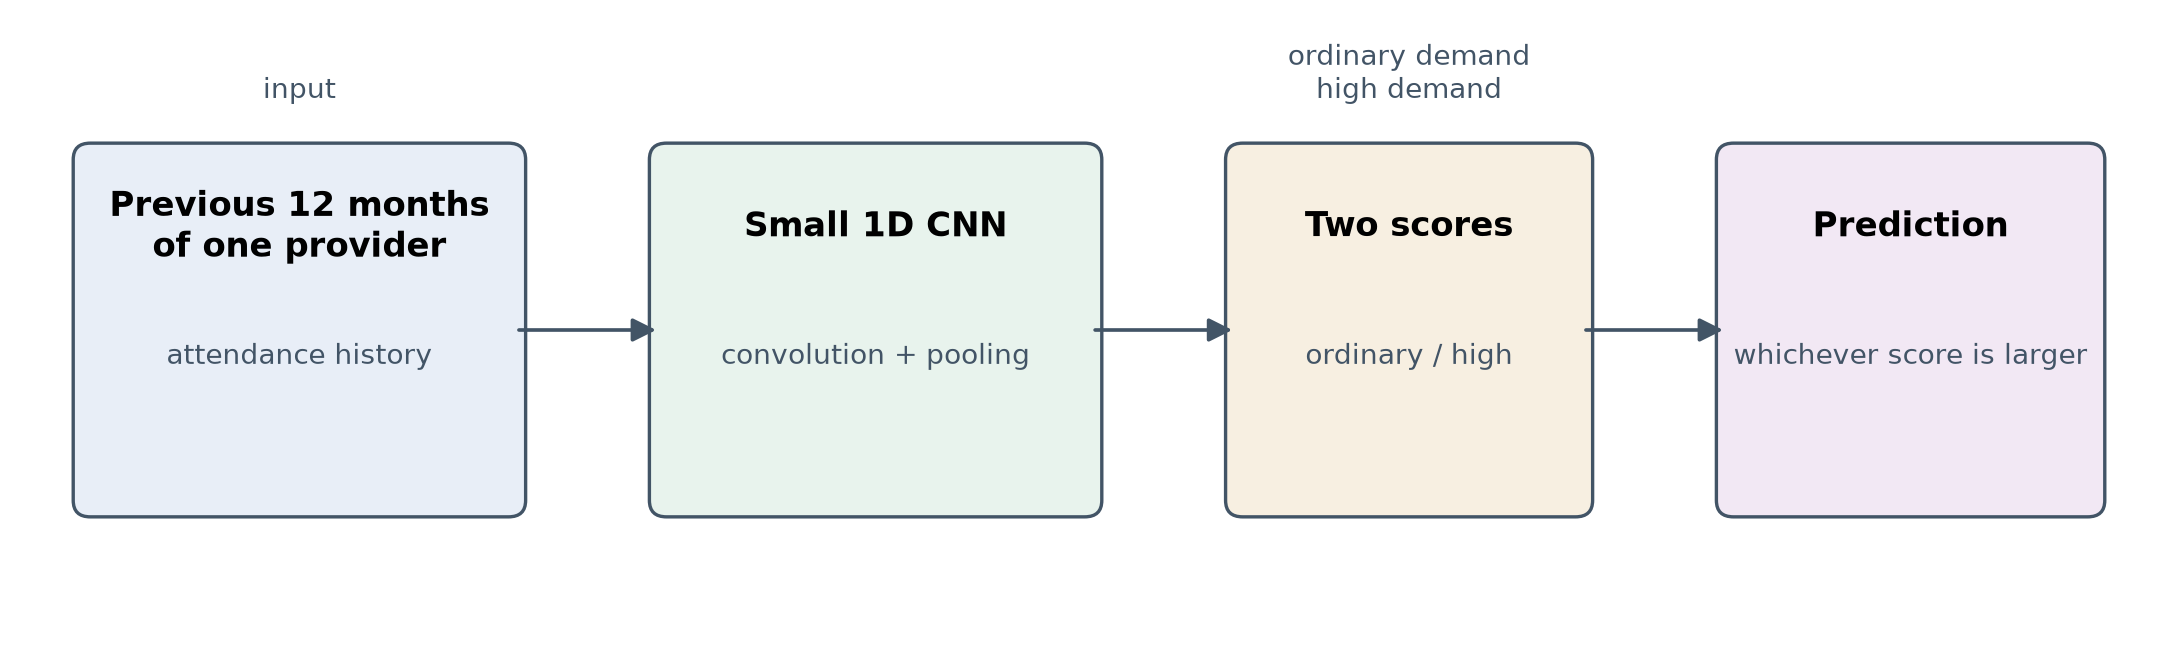
\includegraphics[width=0.94\linewidth]{../figures/report_task.png}
\caption{The prediction task. The model receives the previous twelve months for one provider and produces one score for ordinary demand and one for high demand. The larger score determines the prediction.}
\end{figure}

For a provider $p$ and a month $t$, let $a_{p,t}$ be the number of attendances in that month. The input is the previous twelve values,
\[
x_{p,t} = (a_{p,t-12},\ldots,a_{p,t-1}).
\]
The values are divided by the median of this twelve-month window and one is subtracted. This means that a large hospital is not automatically treated as more likely to have high demand just because it has more attendances. The network sees the recent shape and level relative to the provider's own history.

I labelled the next month high demand when it reached at least the 75th percentile of the same preceding twelve-month window. If $q_{p,t}$ is that percentile, the target is
\[
y_{p,t} = \mathbb{1}\{a_{p,t} \geq q_{p,t}\},
\]
where $\mathbb{1}\{\cdot\}$ is one when the condition is true and zero otherwise. The threshold is calculated only from months available before the prediction date.

\section*{The small neural network}
The model is a deliberately small one-dimensional convolutional neural network. Rather than looking at all twelve months at once, the convolution moves along the history looking at short groups of neighbouring months. It uses the same learned weights at each position, which lets it recognise similar patterns wherever they appear. It produces eight sets of intermediate values. ReLU removes negative values, and average pooling reduces each set to one number. I call these eight numbers the hidden activations: they are the model's internal summary of which short patterns it noticed in the input.

The final linear layer turns those eight activations into two scores. Each score is a weighted combination of the activations plus a bias, so the final layer decides how much each detected pattern should count for ordinary or high demand. There are 50 trainable parameters in total: 32 in the convolution and 18 in the final layer. I chose this architecture because it is small enough to inspect and edit, while still being a reasonable way to recognise short patterns in a time series.

I trained the CNN for 250 full-batch Adam updates using class-weighted cross-entropy. The weights were fitted only on the chronological training period. I selected the CNN's decision threshold on the validation period, then used that fixed threshold for the final test check. Logistic regression received the same twelve normalised values, and seasonal persistence used the attendance value from twelve months earlier as a simple conventional comparison. I did not search over architectures or repeatedly tune the experiment.

\section*{Was the starting model any good?}
Before thinking about editing, I checked whether the CNN had learned a useful relationship. ROC-AUC is a ranking measure: it asks how often a randomly chosen high-demand month receives a higher predicted probability than a randomly chosen ordinary month. A value of 0.5 is chance, while a larger value means the probabilities contain more useful ordering information.

On the final six-month test period, the provider-level CNN achieved ROC-AUC 0.670. Logistic regression achieved 0.674 and seasonal persistence achieved 0.565. The CNN therefore learned a measurable signal, although it was not a superior hospital forecasting model. Its purpose here was to provide a competent, inspectable neural model with a specific weakness to investigate.

\begin{figure}[htbp]
\centering
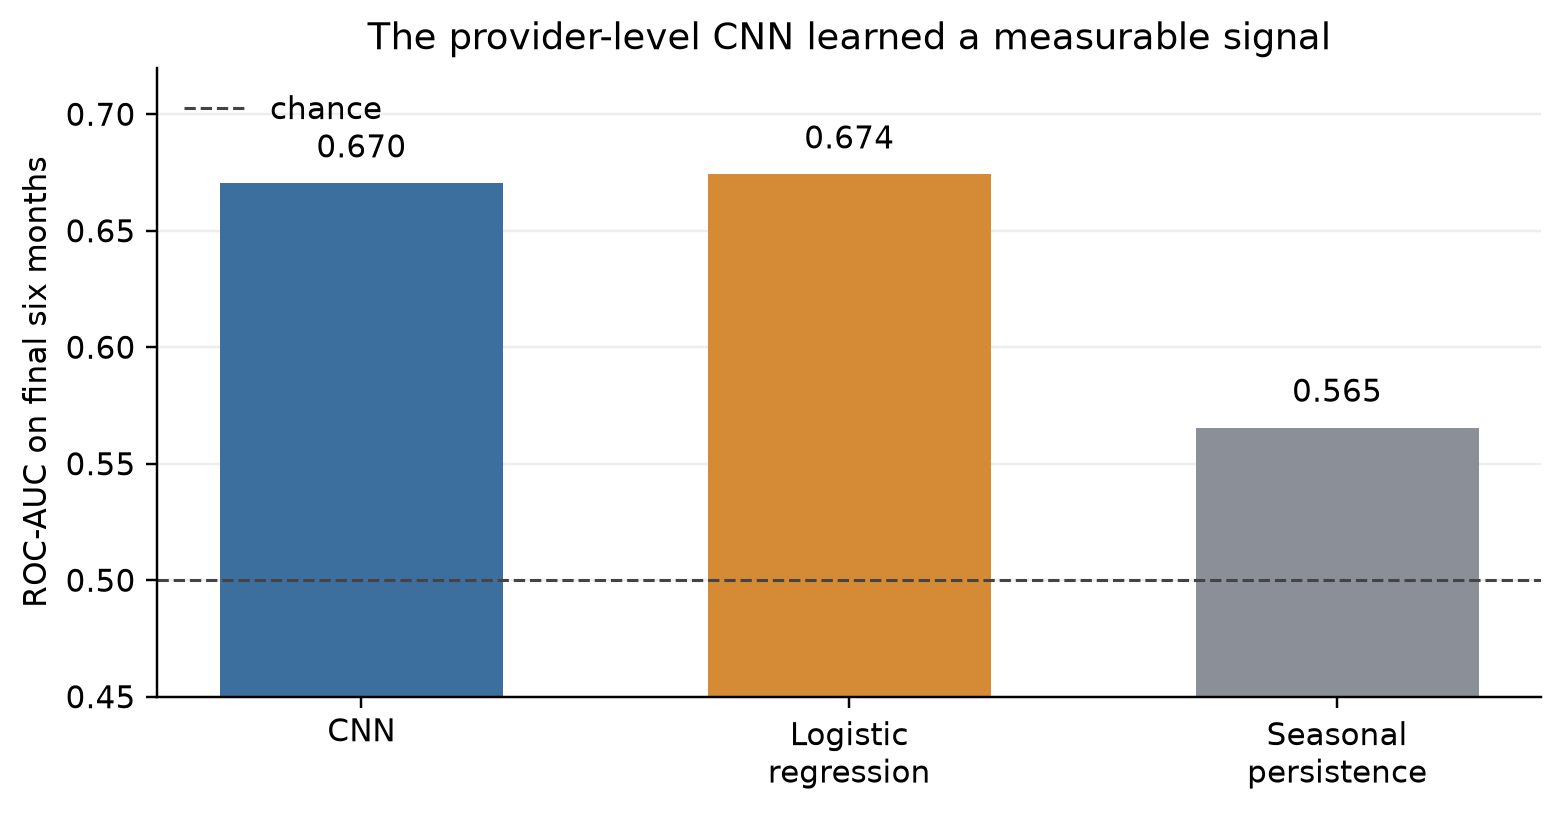
\includegraphics[width=0.78\linewidth]{../figures/report_baseline_comparison.png}
\caption{Held-out ROC-AUC for the provider-level CNN and two simpler baselines. The neural model is meaningfully above chance, but logistic regression is slightly better on this measure.}
\end{figure}

\section*{Finding a repeated mistake}
I next looked only at training and validation examples, leaving the final test period out of the search for a failure pattern. I found that the CNN often missed unusually busy months when attendance had been flat or falling over the preceding six months. More precisely, I compared the mean of the most recent three months with the mean of the three months before them.

There were 409 high-demand examples in this group, from 161 providers. The CNN's high-demand recall was 29.6\%, compared with 74.5\% for high-demand months after a recent rise. Recall means the fraction of genuinely high-demand months that the model successfully identifies. The difference appeared in both the training and validation periods, rather than being caused by one provider or one isolated month.

One example was provider AAH in July 2025. The twelve normalised inputs were
\[
\texttt{(0.201, 0.011, -0.057, -0.086, -0.055, 0.002, 0.097, -0.002, 0.295, -0.018, -0.040, 0.119)}.
\]
The month had 688 attendances, above its preceding-window threshold of 602, but the CNN gave high demand probability 0.440. Its ordinary and high-demand scores were 0.173 and $-0.070$, so ordinary demand still led. The hidden activations were
\texttt{(0.323, 0.365, 0.469, 0.493, 0.421, 0, 0.444, 0.429)}.

\begin{figure}[htbp]
\centering
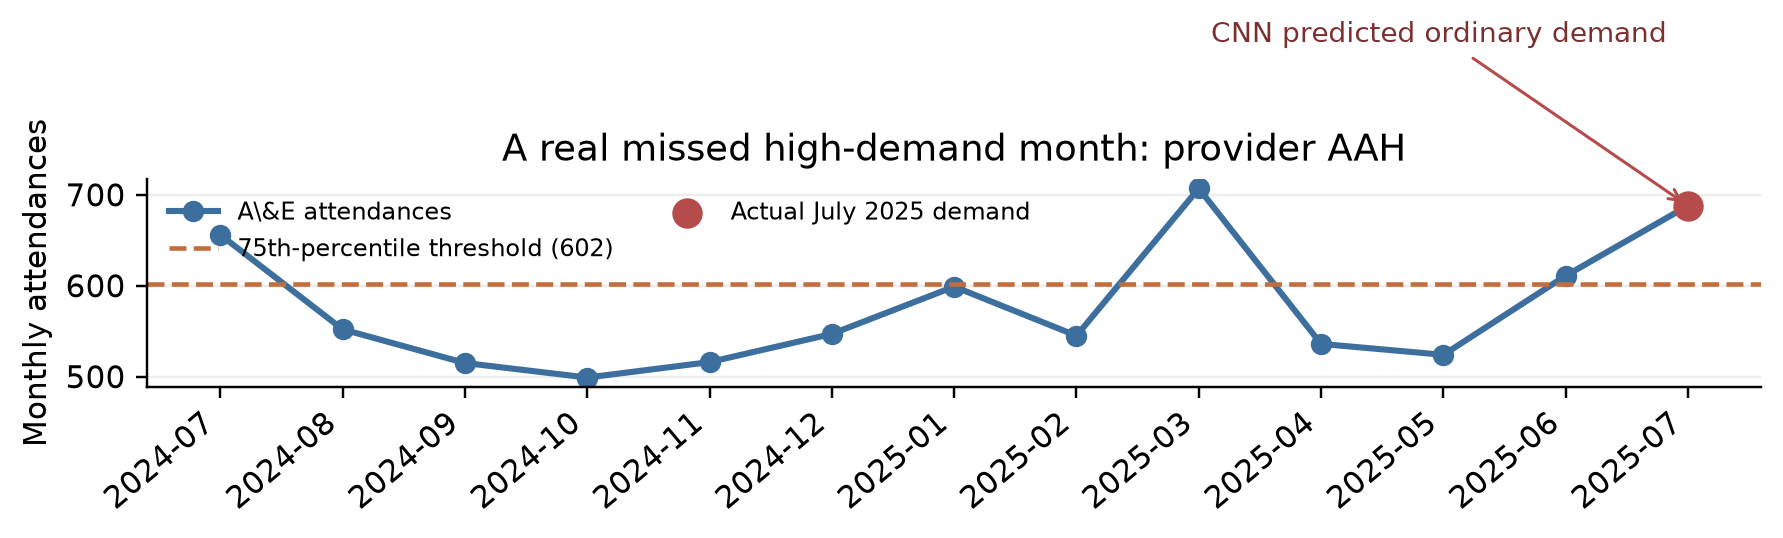
\includegraphics[width=0.89\linewidth]{../figures/report_failure_example.png}
\caption{A real failure from provider AAH. July 2025 was above the provider's preceding-window 75th-percentile threshold, but the CNN still predicted ordinary demand. The preceding history does not contain a clear recent rise.}
\end{figure}

This seemed like a useful behaviour to investigate because it appeared repeatedly and had a simple description. It was not clear that a small edit could repair it. In fact, logistic regression already recalled 69.2\% of these validation cases with 252 false alarms overall, while the CNN recalled 49.5\% with 249 false alarms. I therefore treated weight editing as an experiment, not as the assumed solution.

\section*{Changing the weights mathematically}
The final layer has two rows of weights. I found it easier to think about the difference between the two scores, rather than the scores individually. If the high-demand score is larger, the network predicts high demand. The difference tells me how far it is from changing its mind. For an input with hidden activation vector $h$, the ordinary and high-demand scores are
\[
z_0 = w_0^\mathsf{T}h+b_0, \qquad z_1 = w_1^\mathsf{T}h+b_1,
\]
where $w_0,w_1$ are the two rows of final-layer weights and $b_0,b_1$ are their biases. The classifier chooses the larger score. It is useful to describe the decision using the margin
\[
m = z_1-z_0 = (w_1-w_0)^\mathsf{T}h+(b_1-b_0).
\]
A positive margin favours high demand; a negative margin favours ordinary demand. This equation also explains why a final-layer edit is easy to analyse: changing one weight changes the margin in proportion to the corresponding hidden activation.

I selected one flat-or-falling, genuinely high-demand training example from each of the first 16 providers in sorted provider and date order. These were fixed before the edit. I called this set $T$. I also used all ordinary-demand training examples as a preservation set $N$, so that the edit would be discouraged from simply increasing the high-demand score everywhere. This penalty was not a guarantee that the rest of the model would be preserved; the validation results show that a broad increase could still occur.

If $\Delta$ represents the changes to the 18 editable final-layer scalars, the objective used in the code was
\[
J(\Delta) = \frac{1}{|T|}\sum_{i\in T}\bigl(m_i(\Delta)-m_i(0)\bigr)
 - \lambda\frac{1}{|N|}\sum_{j\in N}\bigl(m_j(\Delta)-m_j(0)\bigr),
\qquad \lambda=1.
\]
The first term rewards a larger high-demand margin on the selected failures. The second term penalises the same margin increase on ordinary training examples. I wanted to stop the edit from simply rewriting the model. The challenge was to see whether a few small changes could make a useful difference. I restricted the edit using
\[
\|\Delta\|_0\leq 8, \qquad \|\Delta\|_\infty\leq 0.10, \qquad \|\Delta\|_2\leq 0.20.
\]
These three conditions mean that at most eight numbers can change, no number can move by more than 0.10, and the total size of the change is limited. The first constraint counts non-zero changes, the second is the largest individual movement, and the third is the Euclidean length of the whole patch.

Because the final-layer scores are linear in these parameters, the objective is linear in $\Delta$. The implementation enumerated every possible support of up to eight parameters and solved the bounded problem for each support, rather than assuming that the largest individual influences must form the best edit. The resulting patch changed eight parameters, reached the full L2 limit of 0.20, and corrected four of the 16 selected training examples.

\begin{figure}[htbp]
\centering
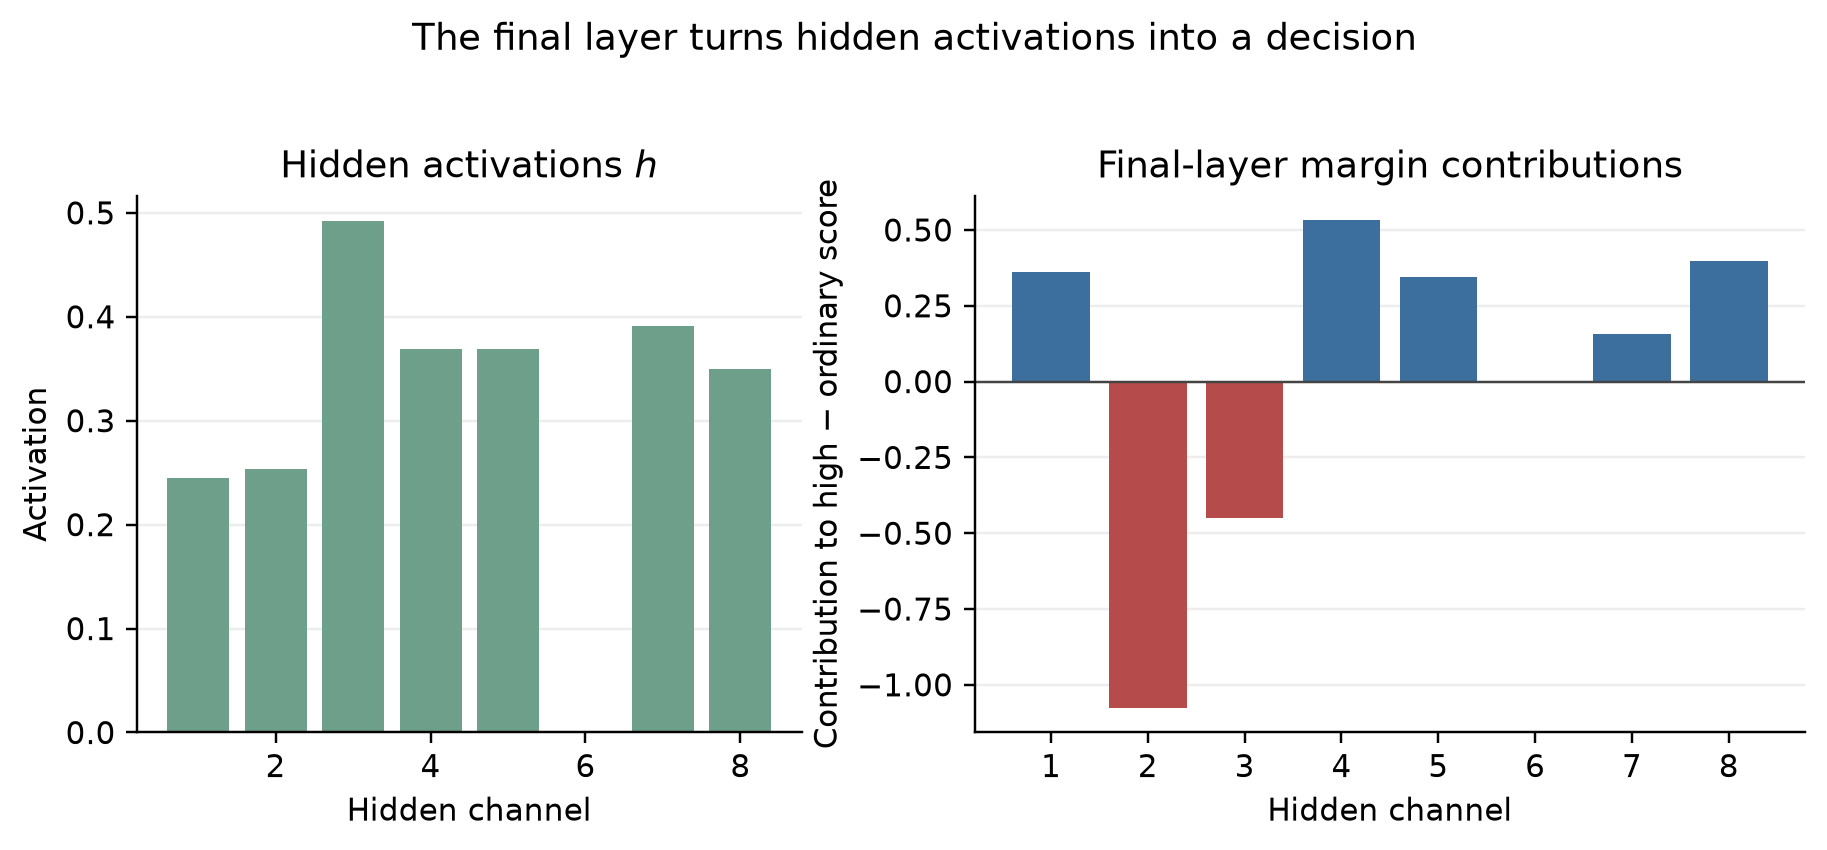
\includegraphics[width=0.88\linewidth]{../figures/report_edit_mechanism.png}
\caption{For one real provider history, the eight hidden activations are combined by the final layer. Each bar on the right is that channel's contribution to the high-demand-minus-ordinary margin. A final-layer edit changes these contributions without retraining the convolutional part of the network.}
\end{figure}

On validation data, the target-pattern recall rose from 49.5\% to 85.0\%. However, false alarms rose from 249 to 493 and balanced accuracy fell from 64.4\% to 57.6\%. The edit had improved the selected direction of the scores, but it had not preserved the rest of the classifier. This was the first important result: improving a numerical objective is not the same as repairing useful behaviour.

\section*{Asking the language model}
I then asked whether a language model could propose a more selective edit. The LLM received the architecture, the final-layer weights and biases, the 16 fixed training failures, their input histories, hidden activations, output scores and labels, and eight predetermined ordinary training examples for context. It received no validation or test results and no analytical patch or analytical outcome.

The request used \texttt{gpt-6.1-sol} with medium reasoning effort. The response had to be a strict JSON patch. The validator permitted only the two final-layer parameters, checked indices and duplicate entries, and enforced the same limits as the analytical experiment. An empty patch was allowed, and the explanation was treated as a hypothesis rather than evidence.

The LLM returned eight changes, all to final-layer weights. The maximum absolute change was 0.09 and the total L2 magnitude was approximately 0.156, so the patch passed validation.

\begin{center}
\small
\begin{tabular}{@{}lrr@{}}
\toprule
Parameter column (zero-based) & Ordinary row change & High-demand row change \\
\midrule
6 & $-0.090$ & $+0.090$ \\
4 & $-0.045$ & $+0.045$ \\
7 & $-0.040$ & $+0.040$ \\
2 & $+0.020$ & $-0.020$ \\
\bottomrule
\end{tabular}
\end{center}

The paired changes were intended to increase the contribution of some hidden channels to the high-demand score while reducing another contribution. The model's explanation was a reasonable hypothesis about the supplied examples, but it could not establish that the same channels would be selective on unseen providers. That had to be checked by evaluation.

\section*{What happened on validation data?}
I evaluated the original model, a threshold change, the analytical edit, the LLM edit and logistic regression on the same 1,080-example validation period. The CNN's original validation-selected threshold was kept for both weight edits. The threshold baseline used 0.5, and logistic regression used its own threshold selected from validation data. False alarms are ordinary-demand examples incorrectly labelled high demand. Balanced accuracy gives equal weight to recall on the two classes, so it falls when extra high-demand predictions are mostly wrong.

\begin{center}
\small
\begin{tabular}{@{}lrrr@{}}
\toprule
Method & Flat/falling recall & False alarms & Balanced accuracy \\
\midrule
Original CNN & 49.5\% & 249 & 64.4\% \\
Threshold 0.5 & 72.0\% & 377 & 62.2\% \\
Analytical edit & 85.0\% & 493 & 57.6\% \\
LLM edit & 79.4\% & 419 & 60.8\% \\
Logistic regression & 69.2\% & 252 & 68.9\% \\
\bottomrule
\end{tabular}
\end{center}

The LLM edit found 85 of the 107 flat-or-falling high-demand validation cases, compared with 53 for the original CNN. That is a real change in classification behaviour. It also produced 419 false alarms instead of 249, however, and overall balanced accuracy fell from 64.4\% to 60.8\%. The analytical edit raised recall even further, but caused still more false alarms. Logistic regression was the strongest of these validation comparisons: it handled the target pattern reasonably well without shifting the decision boundary as widely.

\begin{figure}[htbp]
\centering
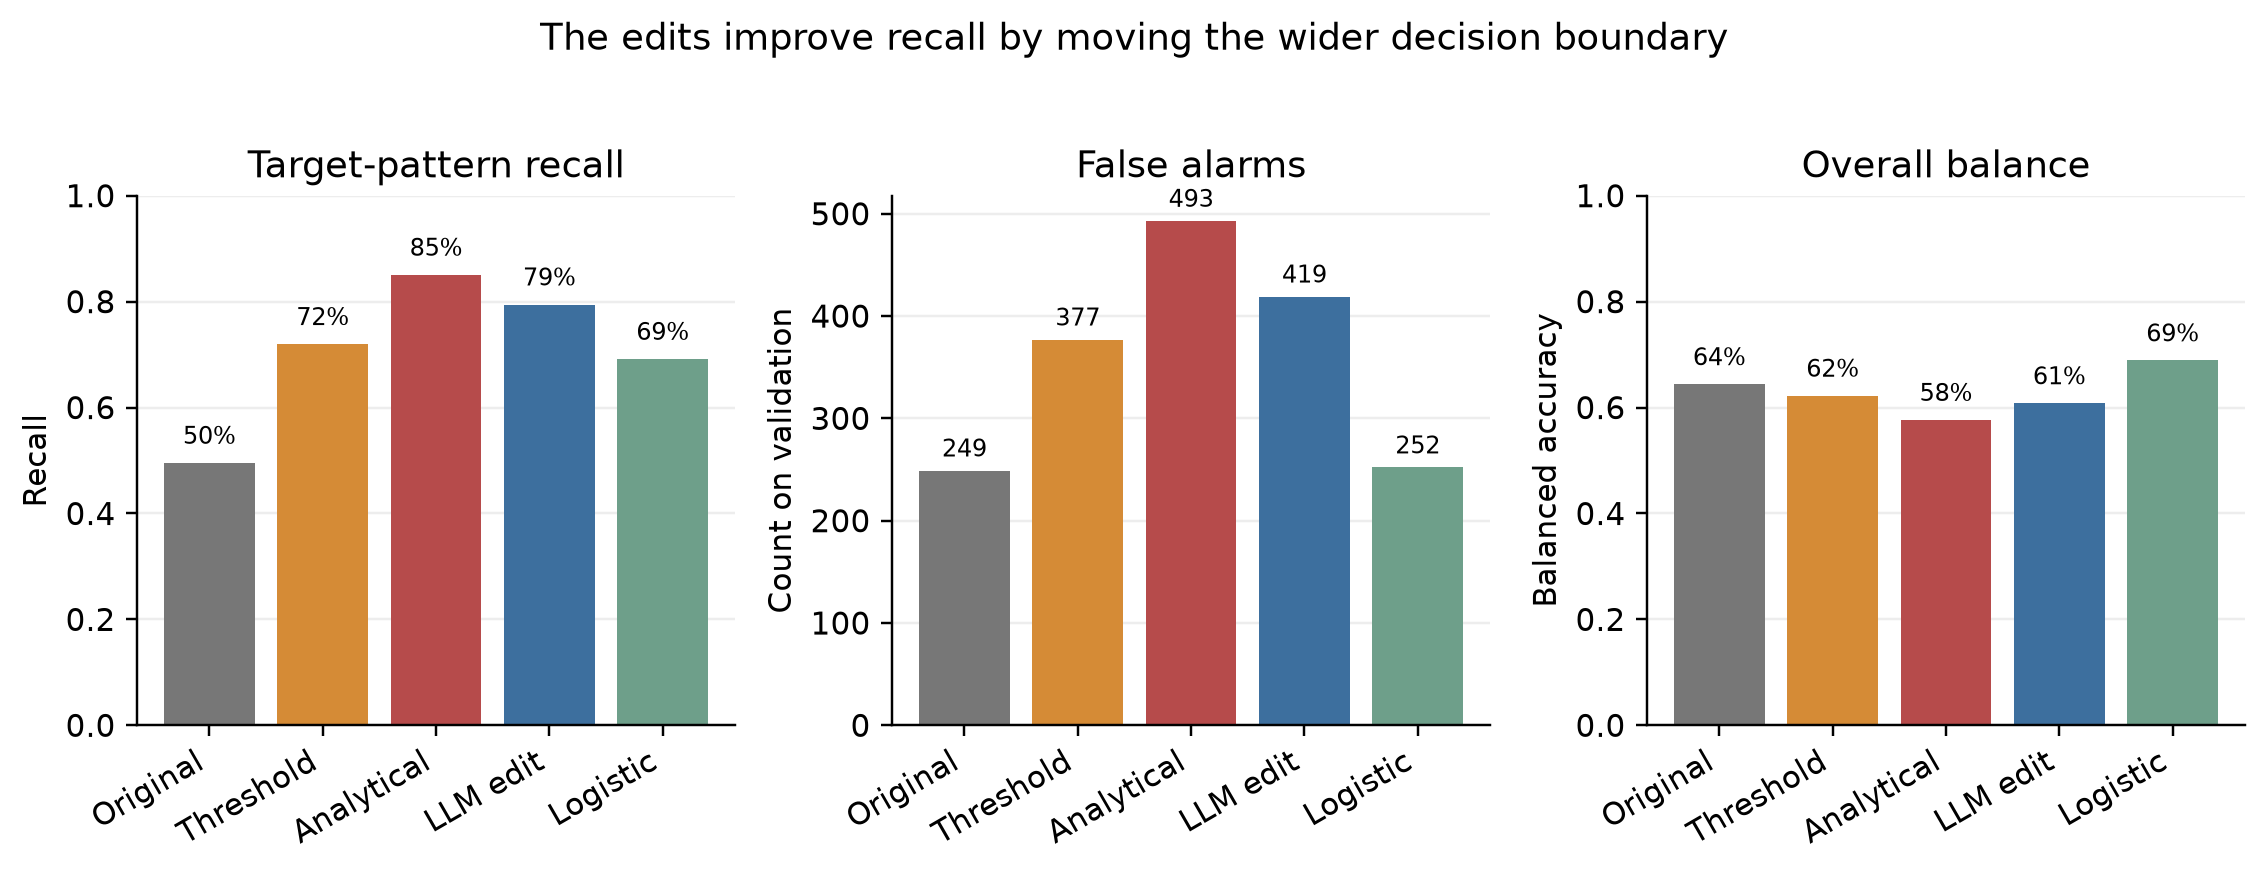
\includegraphics[width=\linewidth]{../figures/report_edit_comparison.png}
\caption{The main comparison on the validation period. Both weight edits improve recall on the selected pattern, but both also create many more false alarms. The LLM edit is somewhat more selective than the analytical edit, but neither improves overall balanced accuracy.}
\end{figure}

The LLM edit therefore did something interesting but not sufficient. It produced a valid, small and interpretable numerical change that moved the desired predictions in the intended direction. It did not discover a selective repair of the network's behaviour. The analytical objective was also specific and limited, so this result does not show that LLMs are generally better or worse than mathematical optimisation for weight editing.

\section*{What I learned}
The useful distinction in this project is between changing a score and repairing a system. The LLM could inspect the small network, choose permitted parameters and make a patch that improved several target predictions. But those parameters also affected many ordinary examples, and the false-alarm cost was too high.

This is one controlled experiment on one small model. It does not show that a language model understands neural networks in a general sense, and it does not establish that direct weight editing is preferable to retraining, threshold adjustment or logistic regression. It does show why an edit needs a preservation test as well as a target test. A change that looks sensible inside the model can still be a poor change to the behaviour people actually care about.

\vspace{.3em}
\small\noindent\textit{Data source:} \href{https://www.england.nhs.uk/statistics/statistical-work-areas/ae-waiting-times-and-activity/}{NHS England A\&E Attendances and Emergency Admissions statistics}. The project was inspired by \href{https://rikiyat.github.io/blog/weight-space-programming/}{Rikiya Takehi's Weight-Space Programming article}; this report is not a reproduction of that work.

\end{document}
